\section{Introduction}
When working with images, it is often usual to use a smaller representation of the original image.
This can be achieved either by scaling down the image or cropping it. This write-up will show, why resizing and cropping are not the best methods to achieve it and introduce better solutions like bidirectional similarity\cite{bisi} and inverse texture synthesis\cite{its}. 

\begin{figure}[h]
\centering
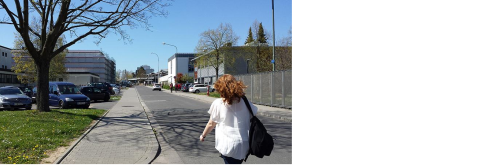
\includegraphics[scale=0.9]{img/ShrinkingCropping}
\caption[blah]{The original image on top shows parts of the University of Mainz with view on
the mensa at the end of street and a person in front. (a) was normally shrinked and (b) was shrinked by using content aware scaling of Adobe Photoshop\footnotemark. (c) is a result of croping, focusing on the mensa.}
\label{Image shrinking}
\end{figure}
\footnotetext{Further reading at Adobe Helpcenter: https://helpx.adobe.com/photoshop/using/content-aware-scaling.html}


\subsection{Shrinking images}
Shrinking or down scaling images is probably the fastest way to get the desired smaller representation of the image. A big advantage of shrinking images is that the layout of the images remain as it was before. On the other hand the smaller image loses quality of the resolution and the change of aspect ratio caused distortion. Figure 1 (a) shows a normal down scaled image. As expected the person on it doesn't look like natural anymore because of the distortion.\\
Figure 1 (b) shows another method of image shrinking which uses the paradigma of importance-based scaling where unimportant parts get more down scaled and important parts less. So compared with (a) the person and the tree look way more natural, but the sidewalk disappears because of different scalings.



\subsection{Croping images}
Croping images is another fast way to obatain a smaller representation. Figure 1 (c) shows a croped image. Unlike (a) and (b) the quality of resolution in (c) stays equal, but as clearest disadvantage every information outside the croped area gets lost. \\
For croping also exists a importance-based croping which works well on images with concentrated important regions, so that the lost parts only consists of unimportant informations.\\
The disadvantages of both methods, shrinking and croping, are to heavy for satisfying results. That is why I will introduce two better methods in the next two sections.
